\chapter{Theorie}
	\section{Segmentierung}
		Segmentierung bezeichnet einen Vorgang, bei dem ein Bild nach bestimmten Homogenit�tskriterien in inhaltlich zusammenh�ngende Regionen einzuteilen. Von den verschiedenen Ans�tzen, die das erreichen sollen, befasst sich diese Arbeit mit pixelbasierten Verfahren, bei denen jedem Pixel in einem Bild eine Klasse zugeordnet wird. Man unterscheidet, wie in \cite{UPSNet} beschrieben, semantische Segmentierung, Instanz-Segmentierung und panoptische Segmentierung.
		\subsection{Semantische Segmentierung}
			Bei der Semantischen Segmentierung soll jeder Pixel eine valide Klasse erhalten. Es wird dabei nicht zwischen unterschiedlichen Instanzen einer Objektklasse unterschieden. Wenn beispielsweise auf einem Bild zwei Fahrzeuge zu sehen sind und bei der Segmentierung die Klasse "Fahrzeug" zugeteilt werden soll, erhalten die Pixel beider Fahrzeuge das Label "Fahrzeug". Die Anzahl valider Klassen bleibt somit bei jeden prozessierten Bild gleich.
		\subsection{Instanz-Segmentierung}
			Im Gegensatz zur semantischen Segmentierung werden bei der Instanz-Segmentierung nur z�hlbare Objekte betrachtet und deren Instanzen ber�cksichtigt. �bertragen auf vorheriges Beispiel w�rden die Pixel des einen Fahrzeug ein Label wie "Fahrzeug1" und die des anderen analog "Fahrzeug2" erhalten.  
		\subsection{Panoptische Segmentierung}
			Die panoptische Segmentierung stellt eine Kombination der vorherigen Segmentations-Arten dar. Z�hlbare Objekte werden demnach nach dem Prinzip der Instanz-Segmentierung und amorphe nach dem der semantischen Segmentierung segmentiert. Die Ergebnisse beider Verfahren werden anschlie�end kombiniert.
	\section{Technologien in DeepLab}
		DeepLab ist ein von Google entwickeltes, 2015  in \cite{DeepLab1} vorgestelltes Modell f�r semantische Segmentierung. Bei der in \cite{DeepLab2} vorgestellten Methode wird ein Deep Convolutional Neural Network (DCNN) zum Erzeugen einer Score Map benutzt, die anschlie�end mit einem Conditional Random Field (CRF) zur endg�ltigen Ausgabe weiterverarbeitet wird. Das Verfahren wird in Abbildung \ref{fig:DeepLabAblauf} grob dargestellt.
		
		\begin{figure}
			\centering
			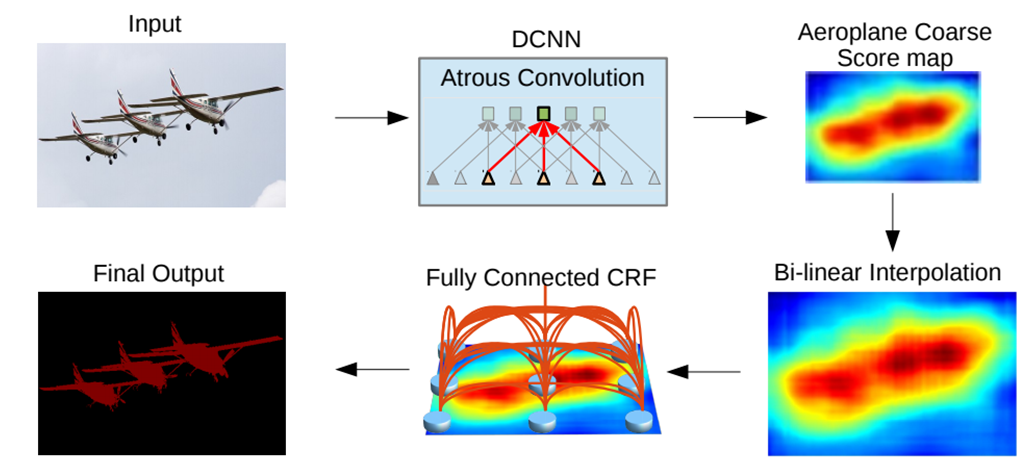
\includegraphics[width = 0.9\linewidth]{img/DeepLabAblauf.png}
			\caption{Grunds�tzliche Funktionsweise von DeepLab}
			\label{fig:DeepLabAblauf}
		\end{figure}  
		\subsection{Deep Convolutional Neural Networks f�r Semantische Segmentierung}
			\subsubsection{Convolutional Neural Networks}
				
			\subsubsection{Anpassungen f�r Semantische Segmentierung}
		\subsection{Atrous Convolution}
		\subsection{Atrous Spatial Pyramid Pooling}
		\subsection{Fully-Connected Conditional Random Fields}
		\subsection{Residual Networks}
	\section{Kamerakalibrierung}
		